%!  pour pdfLatex
\documentclass[a4paper]{article}
%\usepackage[hmargin={1.5cm,1.5cm},vmargin={2.4cm,2.4cm},headheight=13.1pt]{geometry}
\usepackage[a4paper,landscape,twocolumn,
            hmargin=1.8cm,vmargin=2.2cm,headheight=13.1pt]{geometry}

\usepackage[pdftex]{graphicx,color}
\usepackage[pdftex,colorlinks={true},urlcolor={blue},pdfauthor={remy Nicolai}]{hyperref}

\usepackage[T1]{fontenc}
\usepackage[utf8]{inputenc}

\usepackage{lmodern}
\usepackage[frenchb]{babel}

\usepackage{fancyhdr}
\pagestyle{fancy}

\usepackage{floatflt}
\usepackage{maths}

\usepackage{parcolumns}
\setlength{\parindent}{0pt}

\usepackage{caption}
\usepackage{subcaption}

\usepackage{makeidx}

\usepackage[french,ruled,vlined]{algorithm2e}
\SetKwComment{Comment}{\#}{}
\SetKwFor{Tq}{tant que}{}{}
\SetKwFor{Pour}{pour}{}{}
\DontPrintSemicolon
\SetAlgoLined

\usepackage{listings}
\lstset{language=Python,frame=single}
\lstset{literate=
  {á}{{\'a}}1 {é}{{\'e}}1 {í}{{\'i}}1 {ó}{{\'o}}1 {ú}{{\'u}}1
  {Á}{{\'A}}1 {É}{{\'E}}1 {Í}{{\'I}}1 {Ó}{{\'O}}1 {Ú}{{\'U}}1
  {à}{{\`a}}1 {è}{{\`e}}1 {ì}{{\`i}}1 {ò}{{\`o}}1 {ù}{{\`u}}1
  {À}{{\`A}}1 {È}{{\'E}}1 {Ì}{{\`I}}1 {Ò}{{\`O}}1 {Ù}{{\`U}}1
  {ä}{{\"a}}1 {ë}{{\"e}}1 {ï}{{\"i}}1 {ö}{{\"o}}1 {ü}{{\"u}}1
  {Ä}{{\"A}}1 {Ë}{{\"E}}1 {Ï}{{\"I}}1 {Ö}{{\"O}}1 {Ü}{{\"U}}1
  {â}{{\^a}}1 {ê}{{\^e}}1 {î}{{\^i}}1 {ô}{{\^o}}1 {û}{{\^u}}1
  {Â}{{\^A}}1 {Ê}{{\^E}}1 {Î}{{\^I}}1 {Ô}{{\^O}}1 {Û}{{\^U}}1
  {œ}{{\oe}}1 {Œ}{{\OE}}1 {æ}{{\ae}}1 {Æ}{{\AE}}1 {ß}{{\ss}}1
  {ű}{{\H{u}}}1 {Ű}{{\H{U}}}1 {ő}{{\H{o}}}1 {Ő}{{\H{O}}}1
  {ç}{{\c c}}1 {Ç}{{\c C}}1 {ø}{{\o}}1 {å}{{\r a}}1 {Å}{{\r A}}1
  {€}{{\euro}}1 {£}{{\pounds}}1 {«}{{\guillemotleft}}1
  {»}{{\guillemotright}}1 {ñ}{{\~n}}1 {Ñ}{{\~N}}1 {¿}{{?`}}1
}

%pr{\'e}sentation des compteurs de section, ...
\makeatletter
\renewcommand{\thesection}{\Roman{section}.}
\renewcommand{\thesubsection}{\arabic{subsection}.}
\renewcommand{\thesubsubsection}{\arabic{subsubsection}.}
\renewcommand{\labelenumii}{\theenumii.}
\makeatother


\newtheorem*{thm}{Théorème}
\newtheorem{thmn}{Théorème}
\newtheorem*{prop}{Proposition}
\newtheorem{propn}{Proposition}
\newtheorem*{pa}{Présentation axiomatique}
\newtheorem*{propdef}{Proposition - Définition}
\newtheorem*{lem}{Lemme}
\newtheorem{lemn}{Lemme}

\theoremstyle{definition}
\newtheorem*{defi}{Définition}
\newtheorem*{nota}{Notation}
\newtheorem*{exple}{Exemple}
\newtheorem*{exples}{Exemples}


\newenvironment{demo}{\renewcommand{\proofname}{Preuve}\begin{proof}}{\end{proof}}
%\renewcommand{\proofname}{Preuve} doit etre après le begin{document} pour fonctionner

\theoremstyle{remark}
\newtheorem*{rem}{Remarque}
\newtheorem*{rems}{Remarques}

%\usepackage{maths}
%\newcommand{\dbf}{\leftrightarrows}

%En tete et pied de page
\lhead{Informatique}
%\chead{Introduction aux systèmes informatiques}
\rhead{MPSI B Hoche}
\lfoot{\tiny{Cette création est mise à disposition selon le Contrat\\ Paternité-Partage des Conditions Initiales à l'Identique 2.0 France\\ disponible en ligne http://creativecommons.org/licenses/by-sa/2.0/fr/  
} 
\rfoot{\tiny{Rémy Nicolai \jobname \; \today } }
}
\makeindex

%En tete et pied de page
\lhead{Cours IPT}
\chead{Cours 9: Introduction aux bases de données. le 09/05/18}
\begin{document}
\section{Présentation}
Une \emph{base de données relationnelle} est un système de gestion de données. L'objet de ce cours est d'introduire aux concepts élémentaires de tels systèmes.\newline
Les deux fonctions principales de tout système de gestion de données sont :
\begin{center}
 Lire (extraire des informations) \hfill \'Ecrire (insérer ou modifier des informations)
\end{center}
Les \emph{tables} sont les objets fondamentaux sur lesquels les données sont écrites. Elles rassemblent des données qui partagent une même structure. Les \emph{requêtes} sont des programmes agissant sur les tables. Elles sont écrites dans un langage particulier le \emph{SQL} (Structured Query Langage).\newline
Il existe d'autres systèmes de gestion de données: des tableaux (tratés par des logiciels nommés \emph{tableurs}),
des structures hierarchisées (systèmes de fichiers, ldap (Lightweight Directory Access Protocol)), des structures non relationnelles (noSQL, graphDataBase) pour manipuler de plus grandes quantités d'informations.
  
\section{Tables}
\subsection{Dictionnaire}
Comme on dispose d'une certaine habitude des tableaux, on peut les utiliser pour présenter les bases de données. Fondamentalement, une base de données relationnelle est une collections de tableaux qu'il est possible de relier entre eux. Précisons un dictionnaire entre les deux vocabulaires. 
\begin{center}
\begin{tabular}{l|l}
Collections de tableaux & Base de données relationnelle \\ \hline
 tableau & relation ou table \\
 ligne & enregistrement \\
 identifiant de colonne & attribut \\
 type d'une valeur d'une colonne & domaine de l'attribut
\end{tabular}
\end{center}
Des exemples de domaines d'attribut (types pour une colonne) : integer (plusieurs sortes petits ou grands), booléen, date, chaîne de caractêres (longueur fixée), texte (chaîne de caractères de longueur non fixée).
Il n'est pas forcément obligatoire de déclarer un type pour un attribut mais cela permet en général d'accéler les requêtes.\newline
\index{schéma de relation} Le \emph{schéma de relation} est la suite des déclarations des domaines pour chaque attribut (des types pour chaque colonne).\newline
\index{clé primaire}Une \emph{clé primaire} est un attribut particulier qui prend des valeurs différentes pour chaque enregistrement. Une valeur de clé primaire correspond à donc \emph{un seul enregistrement} dans une table et permet de le repérer.

On peut aussi utiliser (dans une certaine mesure) le vocabulaire ensembliste pour parler des bases de données. Une table ressemble à un ensemble dont les éléments sont les enregistrements. Ils partagent la même structure (ce qui n'a pas de sens pour les éléments d'un ensemble). Notons aussi que, en principe, il est possible d'avoir plusieurs fois le même enregistrement dans une table ce qui n'a pas de sens pour un ensemble. Toutefois, c'est une mauvaise pratique. Pour l'éviter, on s'attachera à introduire une clé primaire dans chaque table.

\subsection{Exemple}
La base proposée est formée de deux tables téléchargées depuis le site \href{http://www.data.gouv.fr}{data.gouv.fr}.
Ces tables étaient au format csv (Coma Separated Value). Elles ont été traduites dans le bon encodage (utf8) puis tronquées et insérées dans une base de données nommée \og cours\_2018\fg~ où elles sont désignées par \og AOC\fg~ et \og musees\fg. \newline
On utilise une base de données au travers d'une architecture client-serveur. Ici : un serveur de base de données (MariaDb), un serveur web (apache), une interface d'accès au serveur de bases de données (phpMyAdmin).\newline
La figure \ref{fig:aoc} reproduit une fenêtre présentant la structure de la table \og AOC\fg.
\begin{figure}[h]
  \centering
  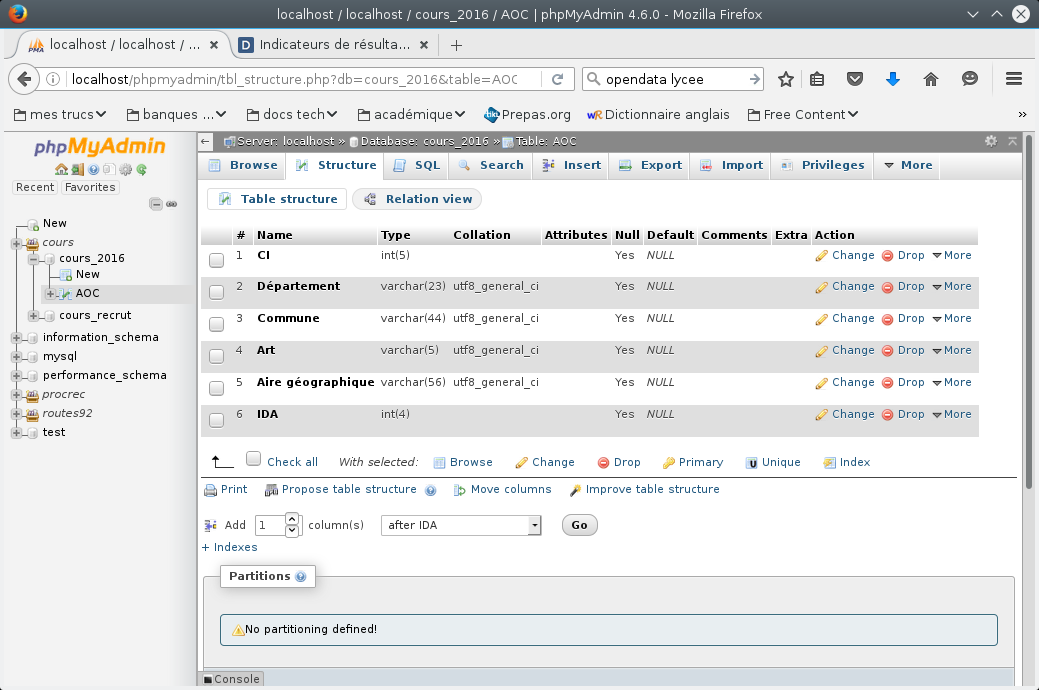
\includegraphics[width=10cm]{./introbdd_aoc.png}
  \caption{structure d'une table - schéma de relation}
  \label{fig:aoc}
\end{figure}


\section{Requêtes}
La figure \ref{fig:requete} présente une \emph{requête} pour extraire (sélectionner) de l'information. Il existe plusieurs dialectes de SQL suivant les vendeurs de bases, ici la syntaxe est minimale et devrait toujours fonctionner.
\subsection{Sélection sans jointure}
\begin{figure}[h]
  \centering
  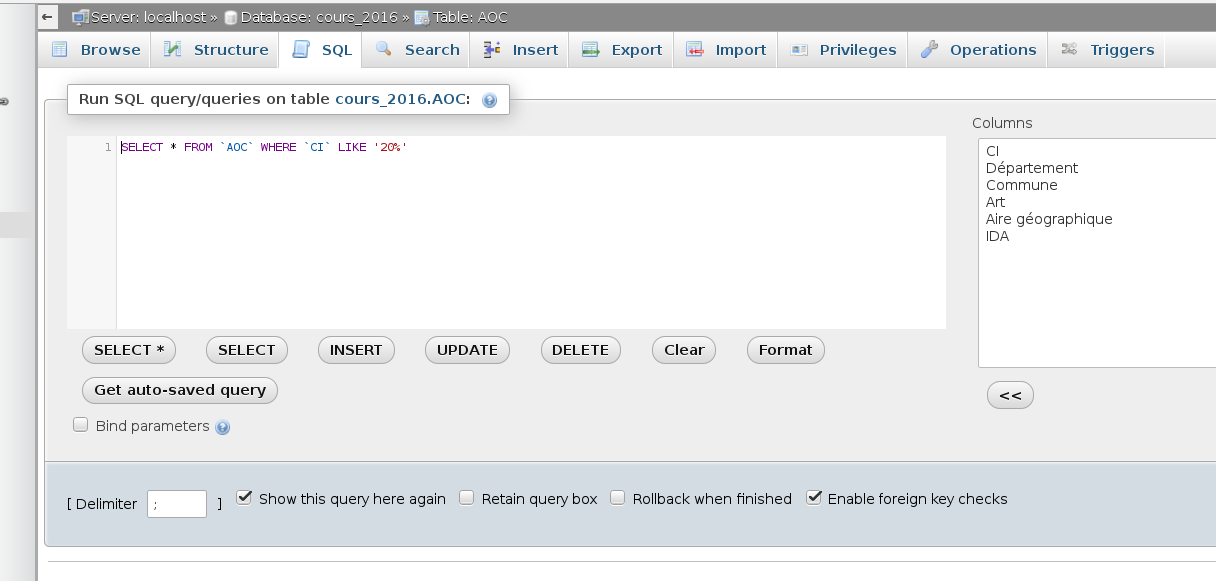
\includegraphics[width=10cm]{./introbdd_requete.png}
  \caption{fenêtre de requêtes}
  \label{fig:requete}
\end{figure}
Examinons (de gauche à droite) le texte de la requête \footnote{Bien noter que l'on peut aller à la ligne et indenter comme on veut}.
\begin{itemize}
  \item Mot réservé \verb|SELECT|. Les majuscules ne sont pas obligatoires mais conseillées.
  \item Liste d'attributs séparés par les virgules. Ils n'ont pas à être dans le même ordre que dans le schéma. Si seulement certains attributs sont demandés sont demandés, on dit que l'on fait une \emph{projection} de la table. Le caractère \verb|*| signifie tous les attributs de la table. On peut combiner les attributs avec des opérations (concaténation \verb|CONCAT()| pour les types chaînes, opération numériques pour les types numériques) ou les composer par des fonctions. La syntaxe de ces opérations dépend du modèle de base. On peut définir un alias pour le nom de l'attribut avec \verb|AS| suivi du nom de l'alias.
  \item Mot réservé \verb|FROM|. Il est suivi par le nom de la base d'où on extrait les enregistrements (entre des guillemets obliques \verb|` `|).
  \item Clause \verb|WHERE | non obligatoire suivie d'une combinaison booléenne de conditions reliées par les opérateurs \verb|AND| , \verb|OR|.
  \item On peut grouper les enregistrements par le mot clé \verb|GROUP BY| suivi d'un nom de colonne. Cela est utile si on a ajouté une fonction du type \verb|COUNT()| dans la liste de ce qui est affiché
  \begin{verbatim}
   SELECT `Aire géographique`, COUNT(`Aire géographique`) AS nb 
    FROM `AOC` GROUP BY `Aire géographique` ORDER BY nb DESC
  \end{verbatim}
  \item On peut ranger par ordre croissant ou décroissant suivant un attribut avec \verb|ORDER BY | nom d'attribut \verb|ASC| ou \verb|DESC|.
\end{itemize}
Exercice. Présenter la colonne du nombre d'AOC par aire géographique par ordre alphabétique de l'aire ou par ordre décroissant du nombre de produits.

\subsection{Jointures}
Les \emph{jointures} lient plusieurs tables. Elles donnent leur puissance aux bases de données en permettant de croiser les informations.\newline
La jointure basique de deux tables forme une nouvelle table virtuelle qui est un produit cartésien des deux. Chaque enregistrement de la jointure est de la forme $(e_i,e'_j)$ où $e_i$ est un enregistrement de la première table et $e'_j$ de la seconde. Comme les tables comportent quelques milliers d'enregistrements cela donne une structure trop grande pour être utile.\newline
En fait, on joint les tables \emph{sur des attributs particuliers} dont des valeurs égales sont présentes dans les deux tables.
\begin{verbatim}
  SELECT * FROM `AOC` JOIN `musees` ON `AOC`.`CI` = `musees`.`CP`
\end{verbatim}
Cela limite la jointure aux enregistrements $(e_i,e'_j)$ pour lesquels les valeurs des attributs de $e_i$ et $e'_j$ sur lesquels se font la jointure sont égaux.\newline
Le reste de la syntaxe de \verb|SELECT| présentée au dessus reste valable.

\subsection{Fonctions d'agrégation}
Les fonctions d'agrégation calculent leurs valeurs à partir de \emph{l'ensemble} des données renvoyées par une requête.\newline
Les exemples suivants présentent la syntaxe des principales fonctions 
\begin{itemize}
  \item le nombre d'enregistrements : \texttt{COUNT(*)}.
  \item le nombre de valeurs distinctes d'un attribut : \texttt{COUNT( DISTINCT nomAttrib)}
  \item la somme des valeurs d'un attribut : \texttt{SUM( nomAttrib)}
  \item la plus grande ou la plus petite des valeurs d'un attribut : \texttt{MAX( nomAttrib)}, \texttt{MIN( nomAttrib)}.
\end{itemize}


\end{document}
